\documentclass[14pt,dvipdfmx,uplatex]{beamer}
\usetheme{Madrid}
\setbeamertemplate{footline}[page number]{}
\beamertemplatenavigationsymbolsempty
\usepackage{mypresentation}
\usepackage[noalphabet]{pxchfon}
\input{jpncolor}

%\setgothicfont{migmix-2p-bold.ttf}
\setgothicfont{RoNOWStd-GE.otf}
\setxboldgothicfont{RoNOWStd-GE.otf}
%\setminchofont{migmix-2p-bold.ttf} % 本文
\mathversion{bold}

\setbeamerfont{title}{size=\HUGE{24}{34},family={\yasagoth}}
\setbeamerfont{frametitle}{size=\HUGE{14}{24},series={\yasagoth}}
\setbeamerfont{frametext}{size=\HUGE{14}{24},series={\yasagoth}}
\setbeamertemplate{frametitle}[default][left]
\setbeamertemplate{itemize items}[triangle]
\setbeamertemplate{enumerate items}[default]
\newenvironment{grayenv}{\only{\setbeamercolor{local structure}{fg=10gray}}}{}

\setbeamercolor{background}{bg=white}
\setbeamercolor{author}{fg=black}
\setbeamercolor{date}{fg=black}
\setbeamercolor{title}{fg=white, bg=kachi}
\setbeamercolor{frametitle}{fg=white}
\setbeamercolor{normal text}{fg=black}
\setbeamerfont{normal text}{family=\rmfamily, series=\bfseries}
\setbeamercolor{structure}{fg=black}

\makeatletter
\define@key{beamerframe}{t}[true]{% top
  \beamer@frametopskip=.2cm plus .5\paperheight\relax%
  \beamer@framebottomskip=0pt plus 1fill\relax%
  \beamer@frametopskipautobreak=\beamer@frametopskip\relax%
  \beamer@framebottomskipautobreak=\beamer@framebottomskip\relax%
  \def\beamer@initfirstlineunskip{}%
}
\def\header#1{\vskip.5\baselineskip{\large\yasagoth #1}}
\tikzset{
  notice/.style  = { fill=shozyohi, white, 
                     rectangle callout, 
                     rounded corners,
                     callout absolute pointer={#1} }
}
\makeatother

\setlength{\leftmargini}{16pt}
\setlength{\leftmarginii}{16pt}

\edef\0{\string\0}
\DeclareTextCommand{\CarriageReturn}{JY2}{\015}

\title{ネットワーク解説書の作り方 \\ --- 著者と出版社の攻防\ --- \\ 出版社の視点編}
\author{\sffamily 鹿野 桂一郎\\
\bfseries ラムダノート株式会社\\
\small\bfseries \email{k16.shikano@lambdanote.com} \\ 
%\twitter{golden\_lucky} 
}
\date{\sffamily\footnotesize 2020年1月24日\\ 於\, JANOG 45}

\begin{document}
\bfseries\fontseries{b}\selectfont

%{\usebackgroundtemplate{\includegraphics[height=1.1\paperheight]{skyrocket.jpg}}%
\frame{\titlepage}
%}

\setbeamertemplate{background canvas}[vertical shading][bottom=white,top=kachi!15]
\setbeamercolor{frametitle}{bg=kachi, fg=white}
\setbeamercolor{structure}{fg=kachi}

\begin{frame}[t]{\inhibitglue 誰?}
  \sffamily\bfseries
  \begin{itemize}
      \item 鹿野桂一郎
        \begin{itemize}
           \item Twitter:\href{https://twitter.com/golden_lucky}{@golden\_lucky}
           \item GitHub:\href{https://github.com/k16shikano}{k16shikano@github}
           \item Blog:\url{https://golden-lucky.hatenablog.com/}
        \end{itemize}
      \item 版元の編集者として
        \begin{itemize}
           \item ネットワークとプログラミングの本を主に企画制作
           \item オーム社に約15年(マスタリングTCP/IPとか)\\
              {\small \url{http://note.golden-lucky.net/2015/09/blog-post.html}}
           \item 2015年から出版社「ラムダノート」を立ち上げ\\
              \url{https://lambdanote.com}
        \end{itemize}
      \item 雇われの編集者として、執筆や制作を請けることも
  \end{itemize}
\end{frame}

\begin{frame}[t]{\inhibitglue 話すことと話さないこと}
  \sffamily
  \begin{itemize}
  \item
    話すこと:\\ 「編集者と本を作るときに役に立つかもしれないこと」
  \item
    話さないこと:\\ 「いい本を書くときの心得」
    \begin{itemize}
      \item 昔、それっぽいことを書きました \\
        \footnotesize 「技術書、それも売れるやつを書きたい人へ、編集者からのアドバイス」\\ \url{https://web.archive.org/web/20170916075801/https://tsuchinoko.dmmlabs.com/?p=2303}
    \end{itemize}
  \end{itemize}
\end{frame}

\begin{frame}[t]{\inhibitglue 編集者の4象限}
  \sffamily
  \begin{center}
  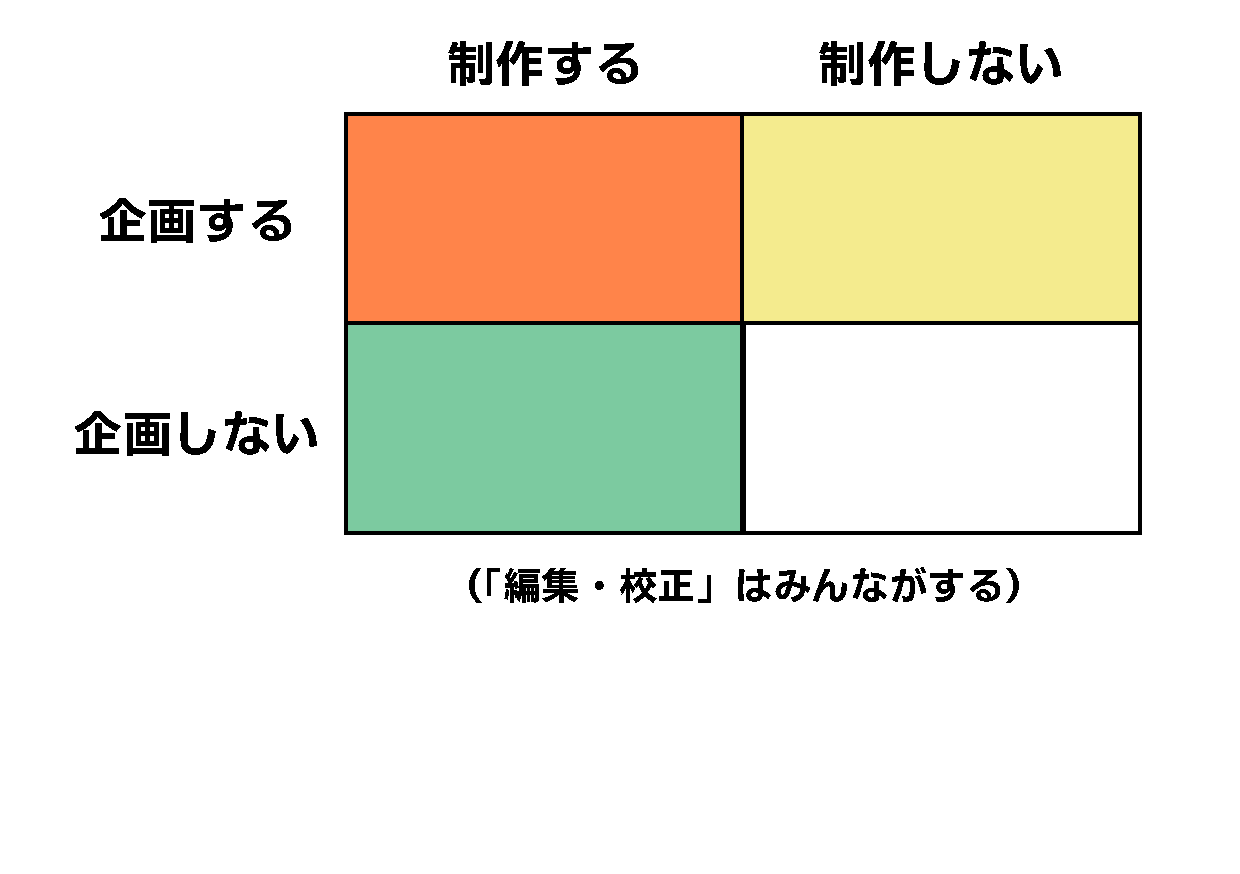
\includegraphics[height=0.9\paperheight]{figures/4segment.pdf}
  \end{center}
\end{frame}

\begin{frame}[t]{\inhibitglue 英語圏ではそれぞれに名前がついている}
  \sffamily\bfseries
  \begin{itemize}
    \item Aquisition Editor
    \item Development Editor
    \item Copyediting Editor
    \item Designer, Typesetter
    \item (Indexer, Advertising Editor, ...)
  \end{itemize}
\end{frame}

\begin{frame}[t]{\inhibitglue 編集者の手懐け方}
    \vfill
  \begin{center}
    \HUGE{19}{28}\color{kachi}\yasagoth
    執筆者にとっての「編集者対策」\\
    as \\
    編集者の「悩み」へのカウンター
  \end{center}
    \vfill
\end{frame}

\begin{frame}[t]{\inhibitglue 編集者にはどんな悩みがあるか}
  \sffamily
    \begin{enumerate}
      \item 企画するネタ
        \begin{itemize}
          \item 書籍が求められている分野は?
          \item 売れそうな書籍は?\\[3ex]
        \end{itemize} 
      \item 著者がいない
        \begin{itemize}
          \item 本を書きたい著者はどこにいる?
          \item 売れそうな著者は?\\[3ex]
        \end{itemize} 
      \item 進捗がまずい
        \begin{itemize}
          \item 著者の進捗
          \item 編集制作の進捗
        \end{itemize}
    \end{enumerate}
\end{frame}

\setbeamertemplate{background canvas}[vertical shading][bottom=white,top=miru!15]
\setbeamercolor{frametitle}{bg=miru, fg=white}
\setbeamercolor{structure}{fg=miru}

\begin{frame}[t]{\inhibitglue 編集者にはどんな悩みがあるか}
  \sffamily
    \begin{enumerate}
      \item 企画するネタ
        \begin{itemize}
          \item 書籍が求められている分野は?
          \item 売れそうな書籍は?\\[3ex]
        \end{itemize} 
      \item<gray@1-> {\color{10gray} 著者がいない}
        \begin{itemize}
          \item {\color{10gray} 本を書きたい著者はどこにいる?}
          \item {\color{10gray} 売れそうな著者は?\\[3ex]}
        \end{itemize} 
      \item<gray@1-> {\color{10gray} 進捗がまずい}
        \begin{itemize}
          \item {\color{10gray} 著者の進捗}
          \item {\color{10gray} 編集制作の進捗}
        \end{itemize}
    \end{enumerate}
\end{frame}

\begin{frame}[t]{\leavevmode\inhibitglue 「企画するネタ」に困っている編集者への対抗策}
  \sffamily
  \begin{enumerate}
      \item 既刊書が多い分野の企画をぶつける
      \item 翻訳書の企画をぶつける
      \item バズっている分野、資格試験の企画をぶつける
      \item 改訂、続編、シリーズの一冊として企画をぶつける
      \item 著者と編集者のマッチングから企画をぶつける
  \end{enumerate}
\end{frame}

\begin{frame}[t]{\inhibitglue 1. 既刊書が多い分野の企画をぶつける}
  \sffamily
  \begin{itemize}
      \item pros.
      \begin{itemize}
        \item 本として成立するネタであることの説明が不要
        \item 既刊書のアラや不評を探すことで構成を立てられる
        \item 関係者に趣旨を説明しやすい
      \end{itemize}
      \item cons.
      \begin{itemize}
        \item 後発であることの実売面での不利
        \item 執筆のモチベーション維持
      \end{itemize}
  \end{itemize}
\end{frame}

\begin{frame}[t]{\inhibitglue 2. 翻訳書の企画をぶつける}
  \sffamily
  \begin{itemize}
      \item pros.
      \begin{itemize}
        \item そもそも完成した書籍がある
        \item 原著の評判から売れ行きを予測しやすい
      \end{itemize}
      \item cons.
      \begin{itemize}
        \item 権利者が多い(原著者、原書出版社、エージェントなどなど)
        \item そのぶんだけコストがかかる
        \item 意外と書下ろしより重労働
      \end{itemize}
  \end{itemize}
\end{frame}

\begin{frame}[t]{\inhibitglue 3. バズっている分野、資格試験の企画をぶつける}
  \sffamily
  \begin{itemize}
      \item pros.
      \begin{itemize}
        \item 潜在的な読者の多さ
      \end{itemize}
      \item cons.
      \begin{itemize}
        \item すぐレッドオーシャン化する可能性
        \item すぐ陳腐化する可能性
        \item 求められる執筆速度
      \end{itemize}
  \end{itemize}
\end{frame}

\begin{frame}[t]{\inhibitglue 4. 改訂、続編、シリーズの一冊として企画をぶつける}
  \sffamily
  \begin{itemize}
      \item pros.
      \begin{itemize}
        \item 既刊の認知度や資産を再利用できる
        \item 既刊への好影響もある
      \end{itemize}
      \item cons.
      \begin{itemize}
        \item 続編や改訂はオリジナルより売れにくい、という経験則
      \end{itemize}
  \end{itemize}
\end{frame}

\begin{frame}[t]{\inhibitglue 5. 著者と編集者のマッチングから企画をぶつける}
  \sffamily
  \begin{itemize}
      \item pros.
      \begin{itemize}
        \item 著者の得手不得手をよく知っている編集者
        \item 編集者の趣向をよく知っている著者
      \end{itemize}
      \item cons.
      \begin{itemize}
        \item 著者の実績と編集者の実績がないと企画も実現も困難
        \item なあなあ(悪い意味で)をどう避けるか
      \end{itemize}
  \end{itemize}
\end{frame}

%* 実績のある著者に新しい本を依頼する
%   + 5年以上企画をやっていないとできない技
%* 長年温めているネタ、というものもある
%   + あるとき偶然に書ける人と知り合ったりする
%   + 10年以上企画をやっているような人はみんなそういうネタ帳を心にもってる

% ネットワーク特有のオペレーションの本をずっとやってきた人が、OSSベースでソフトウェアコンフィグアブルな技術の本の企画を思い付けるとは限らない

% 原稿がきて、読んでみると、いまいち説明だけではクリアでない話があったりする。だいたい実装依存の話だったり、


% NTT NGNをIXとして使えるかどうか、という議論に、教科書にある知識だけでついていけるか。
% BGPの説明からIXの役割を解説して、という説明の仕方になりがち
% 技術で仕事をしている中に入らないと触れられない技術的なアイディアにどうやってキャッチアップするか

% 耳学問からの跳躍
% みんなJANOGとかにきて楽しいのは、現場の人しか知らない話を聽いたりしたいからでは?

% 宣伝色なくプロプラな技術の解説文書を手伝いたい
% マスタリングTCP/IPとかも、最初は物理層からアプリケーション層まで網羅した教科書というコンセプトだったが、だんだん不可能になってきた。上も下も。今日のDWDMの話とか、Ansibleで構成管理とか

\begin{frame}[t]{\inhibitglue 実際には…}
  \sffamily
  \begin{itemize}
    \item 編集者が自分で企画をいろいろ考えることのほうが(たぶん)多い
    \item そのとき、また別の種類の悩みが…
  \end{itemize}
\end{frame}

\setbeamertemplate{background canvas}[vertical shading][bottom=white,top=yamabuki!15]
\setbeamercolor{frametitle}{bg=yamabuki, fg=black}
\setbeamercolor{structure}{fg=kurotobi}

\begin{frame}[t]{\inhibitglue 編集者にはどんな悩みがあるか}
  \sffamily
    \begin{enumerate}
      \item<gray@1-> {\color{10gray} 企画するネタ}
        \begin{itemize}
          \item {\color{10gray}書籍が求められている分野は?}
          \item {\color{10gray}売れそうな書籍は?\\[3ex]}
        \end{itemize} 
      \item 著者がいない
        \begin{itemize}
          \item 本を書きたい著者はどこにいる?
          \item 売れそうな著者は?\\[3ex]
        \end{itemize} 
      \item<gray@1-> {\color{10gray} 進捗がまずい}
        \begin{itemize}
          \item {\color{10gray} 著者の進捗}
          \item {\color{10gray} 編集制作の進捗}
        \end{itemize}
    \end{enumerate}
\end{frame}

\begin{frame}[t]{\leavevmode\inhibitglue 編集者が「著者を探す」ときの方法}
  \sffamily
  \begin{enumerate}
      \item メールやDMで突撃
      \item 技術イベントなどにいく
      \item 紹介してもらう(2ホップ先くらい)
  \end{enumerate}
  \begin{itemize}
      \item いずれの場合も、興味がない話を振られたら即断りましょう
  \end{itemize}
\end{frame}

\begin{frame}[t]{\inhibitglue 1. メールやDMで突撃されたら}
  \sffamily
  \begin{itemize}
    \item 編集者はSNSやブログでの情報発信が多い人に、ダイレクトにアクションすることがある
    \item アクションは、具体的な話のこともあれば、雑な執筆依頼のこともある(編集者しだい)
    \item 具体的な話で誠実そうなら、反応してもらえるとうれしい
    \item 無視される、断られる、などの覚悟はある
  \end{itemize}
\end{frame}

\begin{frame}[t]{\inhibitglue 2. 技術イベントなどで編集者にあったら}
  \sffamily
  \begin{itemize}
    \item いまがまさにそのとき
    \item 著者候補を探すことが目的で参加する場合もあれば、技術情報に触れることが目的で参加する場合もいる
    \item 本を書きたい場合には、気軽に捉まえて話しかけると、参加の目的がどちらであっても喜びます
    \item 本を書きたくない場合でも、技術情報に触れることが目的の編集者なら、技術の話を聴きたがります
  \end{itemize}
\end{frame}

\begin{frame}[t]{\inhibitglue 3. 知り合いから編集者を紹介されたら}
  \sffamily
  \begin{itemize}
    \item 具体的な執筆の相談込みでの紹介か、ただの顔合わせか
    \item 気がのらない話なら遠慮なくスルーで
    \item すでに他の出版社で何か書いている、というエクスキューズは不要です
  \end{itemize}
\end{frame}

\setbeamertemplate{background canvas}[vertical shading][bottom=white,top=toki!15]
\setbeamercolor{frametitle}{bg=toki, fg=black}
\setbeamercolor{structure}{fg=shozyohi}

\begin{frame}[t]{\inhibitglue 編集者にはどんな悩みがあるか}
  \sffamily
    \begin{enumerate}
      \item<gray@1-> {\color{10gray} 企画するネタ}
        \begin{itemize}
          \item {\color{10gray}書籍が求められている分野は?}
          \item {\color{10gray}売れそうな書籍は?\\[3ex]}
        \end{itemize} 
      \item<gray@1-> {\color{10gray} 著者がいない}
        \begin{itemize}
          \item {\color{10gray} 本を書きたい著者はどこにいる?}
          \item {\color{10gray} 売れそうな著者は?\\[3ex]}
        \end{itemize} 
      \item 進捗がまずい
        \begin{itemize}
          \item 著者の進捗
          \item 編集制作の進捗
        \end{itemize}
    \end{enumerate}
\end{frame}

\begin{frame}[t]{\leavevmode\inhibitglue 「進捗」に困っている編集者への対抗策}
  \sffamily
  \begin{enumerate}
      \item 原稿を書く
      \item 組版される前にやれることをすべてやる
      \item 編集者が何をしているか知る
  \end{enumerate}
\end{frame}

\begin{frame}[t]{\inhibitglue 1. 原稿を書く}
  \sffamily
  \begin{itemize}
    \item 編集者は原稿がないと何もできません
    \item 逆に、原稿があると原稿以上の本を作れます\\
    \begin{itemize}
      \item コンテンツの質が上がる、わけではなく、質が変わる
    \end{itemize}
    \item 催促をすべきかどうか、数週間は悩む(個人差があります)
  \end{itemize}
\end{frame}

\begin{frame}[t]{\inhibitglue 2. 組版される前にやれることをすべてやる}
  \sffamily
  \begin{itemize}
    \item \< 「とりあえず組版する」の罠
    \item 組版されたゲラに赤字をたくさん入れる必要がないように原稿を整理するのが編集者のもっとも重要な仕事のひとつ
    \item 組版されたゲラに赤字をたくさん入れて直す、という工程には、省力化の方法がない
    \begin{itemize}
      \item 版管理と自動組版を前提としている出版社は例外
    \end{itemize}
  \end{itemize}
\end{frame}

\begin{frame}[t]{\inhibitglue 3. 編集者が何をしているか知る}
  \sffamily
  \begin{itemize}
    \item 原稿の整理
    \begin{itemize}
      \item 著者と読者のインピーダンスをそろえる作業\\ (型検査と型推論に似ているかも)
      \item 文章としての局所最適解を探す作業\\ (コンパイラの最適化に似ているかも)
      \item 頭から読めるようにする作業(リンカーに似ているかも)
    \end{itemize}
    \item 組版(のための指示)
    \item 装丁デザイン(のための指示)
    \item 販売までのお膳立て(の指示)
    \item 宣伝(の指示)
  \end{itemize}
\end{frame}

\setbeamertemplate{background canvas}[vertical shading][bottom=white,top=sumizome!15]
\setbeamercolor{frametitle}{bg=sumizome, fg=white}
\setbeamercolor{structure}{fg=sumizome}

\begin{frame}[t]{\inhibitglue おまけ:お金の話(口頭のみ)}
  \sffamily
  \begin{itemize}
    \item そもそも本を作るのにいくらかかるのか
    \begin{itemize}
      \item 実際には出版社ごと、本の種類ごとにまちまち
    \end{itemize}
    \item 原価率でいうと…
    \item 定価販売ならではの価格決定の仕組み
    \item 印税の謎
  \end{itemize}
\end{frame}

\begin{frame}[t]{\inhibitglue 想定FAQ}
  \sffamily
  \begin{itemize}
    \item ネットワーク図はどうやって描けばいいの?
    \item 編集者は著者のSNSを監視しているの?
    \item 著者と編集者の生のバトルを見せろ
    \item 出版なんてもうオワコンだろ?
      \begin{itemize}
        \item ブログや同人誌?
        \item セミナー、勉強会、YouTube?
        \item SECCON、NETCONとか?
      \end{itemize}
  \end{itemize}
\end{frame}


\begin{frame}[t]{\inhibitglue バトル例(プロフェッショナル IPv6)}
  \sffamily
  \begin{center}
  \vspace*{-2ex}
  \includegraphics[height=0.85\paperheight]{figures/battle1.png}
  \end{center}
\end{frame}

\begin{frame}[t]{\inhibitglue バトル例(プロフェッショナル IPv6)}
  \sffamily
  \vspace*{-2ex}
  \begin{center}
  \includegraphics[height=0.85\paperheight]{figures/battle2.png}
  \end{center}
\end{frame}


\end{document}
